\subsection{Descripción Circuital}

\subsubsection{Convertidor CC-CC Conmutado}

En la figura \ref{fig:fullbridge} se presenta el circuito completo del convertidor CC-CC conmutado y aislado de tipo puente completo que se utiliza en la plataforma. Consiste de un puente de llaves con diodos en antiparalelo a cada una (de $Q_1$ a $Q_4$). Luego se encuentra un transformador de alta frecuencia que aisla los lados primario y secundario. El puente de diodos del secundario se encarga de generar una forma de onda rectificada, que es luego filtrada por el circuito LC y llevada en forma de corriente continua a la carga $R_L$.\\

\begin{figure}[h]
    \centering
    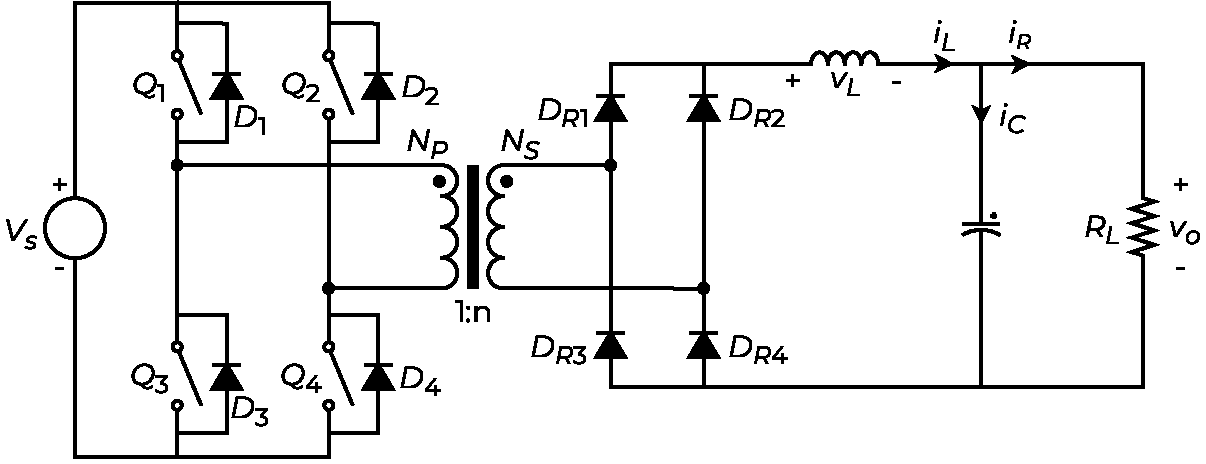
\includegraphics[scale=0.6]{Imagenes/Full Bridge.pdf}
    \caption{Diagrama del convertidor CC-CC de tipo puente completo a utilizar, con todos sus componentes.}
    \label{fig:fullbridge}
\end{figure}

Las funcionalidad de las llaves del primario es llevada a cabo por transistores MOSFET de potencia, cuyo modelo específico se trata más adelante. El lado primario y secundario se conectan a masas distintas ($GND_1$ y $GND_2$ respectivamente), ambas en el lado de potencia de la plataforma.\\

\subsubsection{Circuito Driver}

El circuito driver de la plataforma es el encargado de proveer los pulsos de tensión y corriente necesarios para excitar los MOSFET del puente de transistores y conmutarlos adecuadamente. Esta excitación es comandada por el sistema de control e ingresa por el tercer terminal de cada transistor, en este caso el \textit{gate}. Se observa el cricuito driver para una rama de transistores en la figura \ref{fig:driver}.\\

\begin{figure}[h]
    \centering
    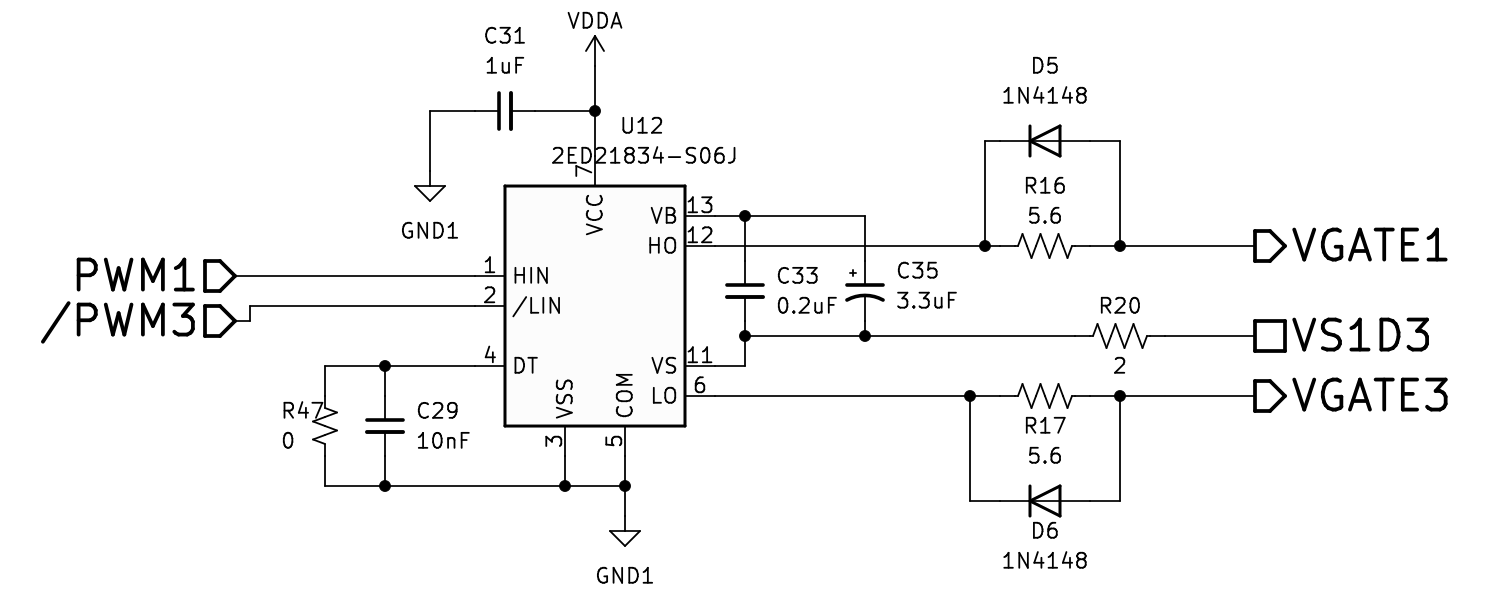
\includegraphics[scale=0.95]{Imagenes/Circuito Driver.png}
    \caption{Circuito de conexión del driver 2ED21834-S06J. El circuito del driver para la otra columna es idéntico.}
    \label{fig:driver}
\end{figure}

Si bien es posible diseñar un sistema de excitación con componentes discretos, resulta más sencillo y confiable utilizar componentes integrados que se encargan de realizar esta función, como el componente U12 que se observa en la figura (los componentes discretos que lo rodean están posicionados y dimensionados según recomendación del fabricante). Al estar encargado de la excitación de los transistores del primario, este circuito se encuentra puesto a tierra mediante la tierra primaria de potencia $GND_1$. Además, como el circuito de arriba es únicamente para una rama, se utiliza otro circuito idéntico para la rama restante de transistores.\\

\subsubsection{Sistema de Medición}

\lipsum[3]\\

\subsubsection{Etapa de Aislación de Señal}

\lipsum[4]\\

\subsubsection{Sistema de Control}

\lipsum[5]\\

\subsubsection{Circuito de Alimentación}

\lipsum[6]\\